\subsection{Environment}
\begin{frame}[containsverbatim, fragile]{Open Street Map}

\only<2>{
        \begin{wrapfigure}[16]{r}{0.375\textwidth}
        \centering
            \vspace{-0.4cm}
            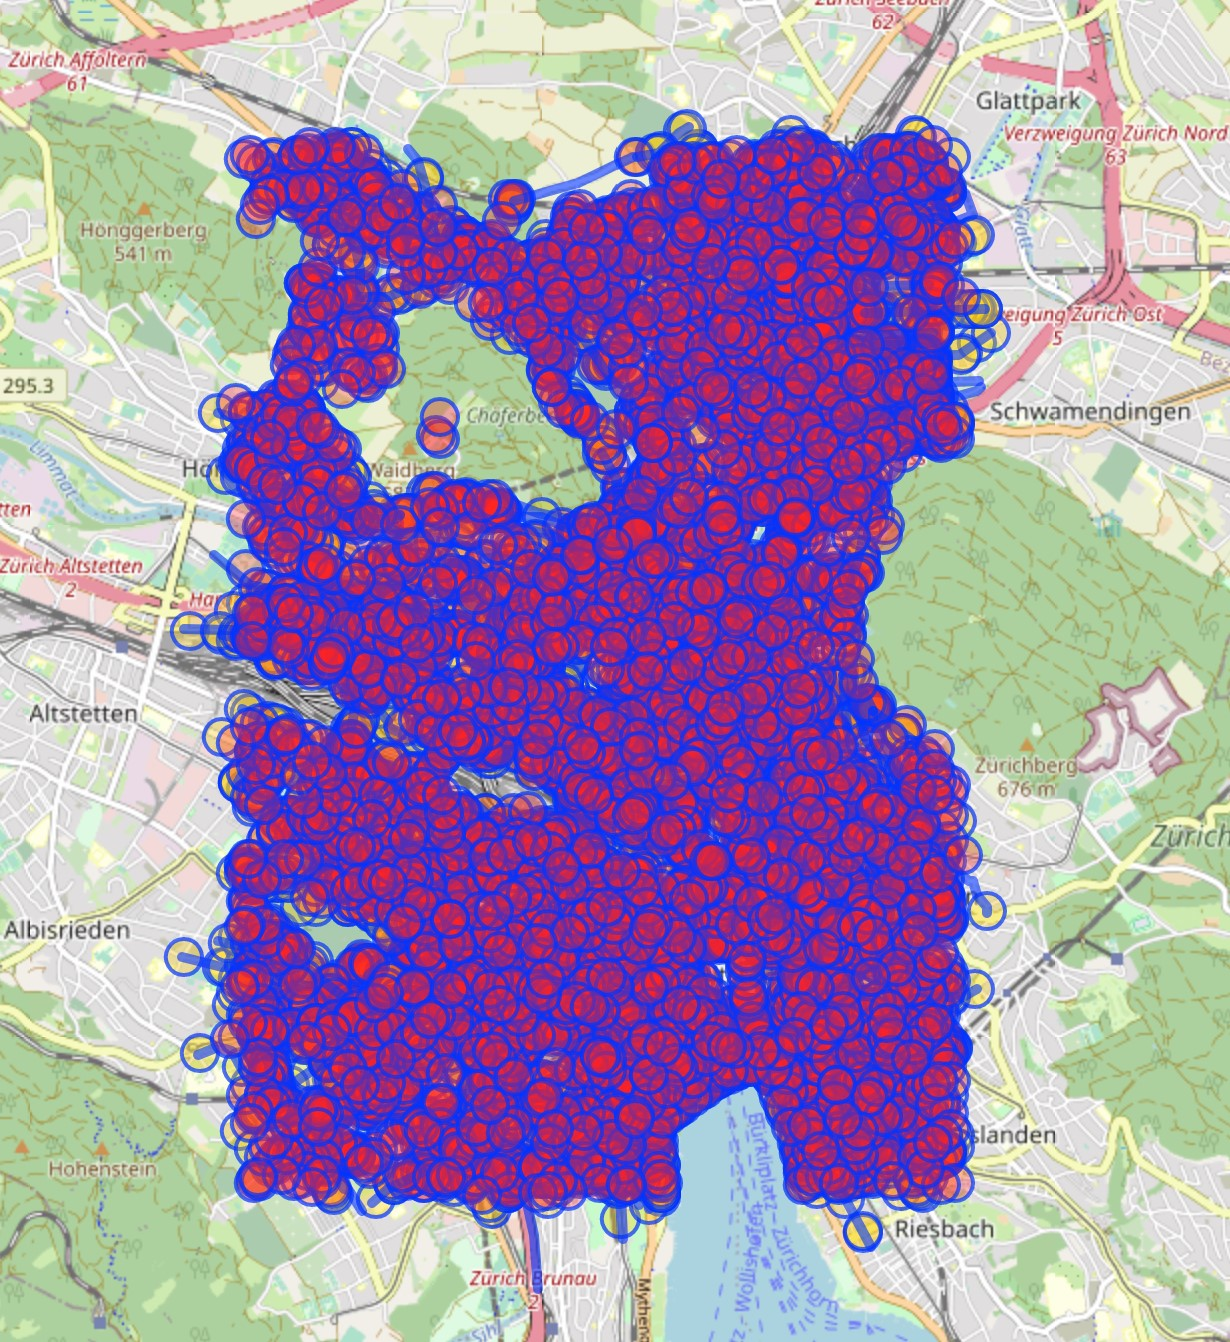
\includegraphics[width=\linewidth]{./Images/road-network.jpeg}
            %\captionsource{Modelled Road Network}{Screenshot taken from Overpass Turbo}\label{network}
        \end{wrapfigure}
 }
 
\begin{lstlisting}[breakindent=0pt, tabsize=1]
[out:json]
[bbox:47.36, 8.50, 47.42, 8.56];
    (
        way[highway=primary];
        way[highway=secondary];
        way[highway=trunk];
        way[highway=tertiary];
        way[highway=service];
        way[highway=residential];
    )->.a;
    (.a;>;);
out;
\end{lstlisting}

\end{frame}


\begin{frame}[containsverbatim, fragile]{Environment}
\only<1->{
    \only<1>{\vspace{-2.4cm}}
    \only<2-5>{\vspace{-1.25cm}}
        Streets and Intersections make up the Model Environment. 
	\begin{multicols}{2}
        \mbox{}
        \only<2->{
        Intersections are characterized by:
        \only<6->{\vspace{-1.8cm}}
            \begin{itemize}
            \setlength\itemsep{1mm}
        	\item<3->[-] IDs
        	\item<4->[-] coordinates
            \item<5->[-] incident streets
		\end{itemize}
        }
        \columnbreak
        \mbox{}
        \only<6->{
         Streets are characterized by:
             \begin{itemize}
                \item<7->[-] ID
         	\item<8->[-] start/end crossing IDs
                \item<9->[-] lanes
                \item<10->[-] length 
                \item<11->[-] speed limit
                \item<12->[-] if present: opposite street ID
		 \end{itemize}
        }
	\end{multicols}
 }
\end{frame}

\subsection{Agents}
\begin{frame}[containsverbatim, fragile]{Agents}

        \begin{wrapfigure}[10]{r}{0.3\textwidth}
        \centering
            \vspace{-0.5cm}
            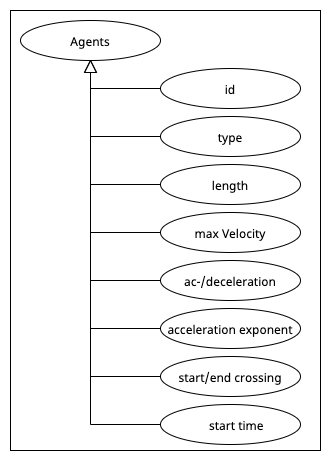
\includegraphics[width=\linewidth]{./Images/Agents.png}
        \end{wrapfigure} 
        
        Agents can be of one of two types, bicycles or cars. Both share the same attribute types but they are chosen out of different intervals.

        \begin{table}[H]
\hspace{-4.5cm}
\begin{tabularx}{0.85\linewidth}{C|C|C}
    \textbf{Attribute} & \textbf{Car} & \textbf{Bike}\\
    \hline
    \textbf{Length} $(m)$ & $[3.5, 5]$ & $[1.5, 2.5]$\\
    \hline
    \textbf{ Max. Velocity} $(km/h)$ & $[100, 250]$ & $[10, 35]$\\
    \hline 
    \textbf {Acceleration} $(m/s^2)$ & $[1.5, 5]$ & $[0.5, 1.5]$\\
    \hline
    \textbf{Deceleration} $(m/s^2)$ & $[2,6]$ & $[1,3]$ \\
    \hline
    \textbf{Acceleration Exponent} & $[8, 12]$ & $[8,12]$
\end{tabularx}
\end{table}

\end{frame}


\subsection{Interaction}
\begin{frame}[containsverbatim, fragile]{Vehicles Behaviour}
	%insert flow chart that describes interactions here
        \begin{figure}
		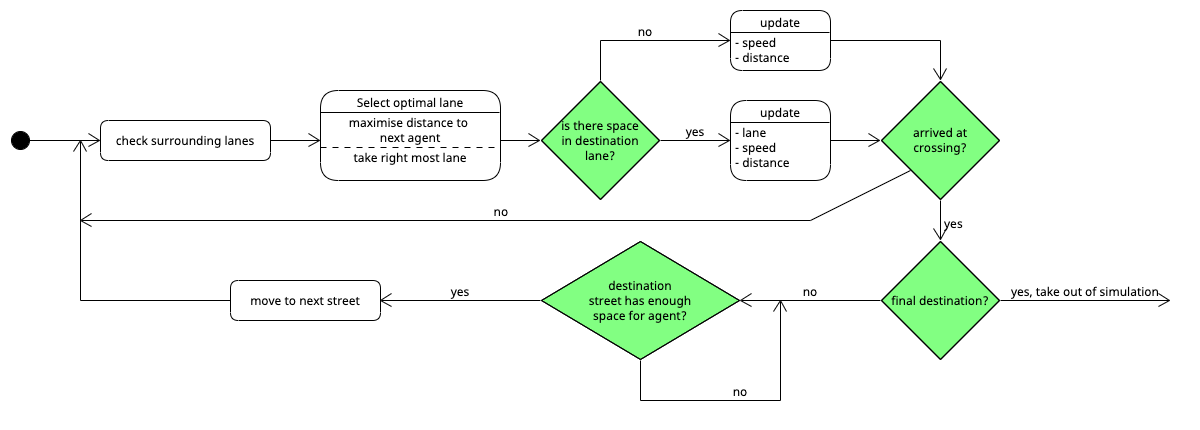
\includegraphics[width=1\textwidth]{Images/AgentBehaviour.png}
	\end{figure}
\end{frame}

\begin{frame}[containsverbatim, fragile]{Differences between Cars and Bikes}
\vspace{-1cm}
        \begin{multicols}{2}
        Bicycles:
        \begin{itemize}
        \setlength\itemsep{1mm}
            \item<2->[-] Bicycles can be on streets and bicycle lanes
            \item<3->[-] Bikes are smaller $\rightarrow$ higher density is possible
            \item<4->[-] Bikes have lower max speeds and acceleration
        \end{itemize}
       
        \columnbreak
        \mbox{}
        \only<4->{
        Cars:
        \vspace{-0.1cm}
            \begin{itemize}
            \setlength\itemsep{1mm}
        	   \item<5->[-] Cars can only be on streets
        	   \item<6->[-] Cars are larger 
                  \item<7->[-] Cars accelerate faster and have a higher max speed
		\end{itemize}
        }
	\end{multicols}
\end{frame}
